% ----------------------------------------
% Geolocation for the Internet of Things using LoRaWAN
% Third Year Project
% Daniel Saul - 2017
% daniel.saul.14@ucl.ac.uk
% ----------------------------------------
% Set up the document class for an article
\documentclass[a4paper]{report}
\usepackage[left=1.0in, right=1.0in, top=1.5in, bottom=1.5in]{geometry}

\setlength{\parskip}{1em}

%\usepackage{savetrees}

% This packages permits using $ \therefore $
\usepackage{amssymb}
\usepackage{graphicx}

% This package allows the use of $ \text{} $
\usepackage{amsmath}

% SI Units, micro etc
\usepackage{siunitx}

% Allows subfigures
\usepackage{subcaption}

% Sort URLs
\usepackage{url}

% Include source code
\usepackage{listings}

% The document title and author
\title{Multilateration-based localization of devices\\within a LoRaWAN network}
\author{Daniel Saul\\University College London\\ \\Supervisor: Dr Miguel Rio}

% Document header
\usepackage{fancyhdr}
\pagestyle{fancy}
\fancyhead[R]{}
\renewcommand{\chaptermark}[1]{%
    \markboth{\MakeUppercase{%
    \chaptername\ \thechapter.%
    \ #1}}{}}
\fancyhead[L]{\leftmark}
\renewcommand{\headrulewidth}{0pt}


% Begin the document
\begin{document}
    \maketitle

% Insert the abstract for the document here
\pagestyle{fancy}

\begin{abstract}

  The Internet of Things is growing at a tremendous rate and with it the need for location estimates of connected devices, particularly in Low Power Wide Area Networks which provide long range communications to low cost and low power devices. Ensuring low power consumption of such devices necessitates alternatives to using a GNSS system such as GPS. This report therefore looks at positioning techniques that might be used with one such network, LoRaWAN. Hardware is built that includes a GPS receiver and LoRa transceiver to gather measurements and ultimately used to evaluate the feasibility of using multilateration to find position estimates of nodes from the Time Difference of Arrival of signals at multiple gateways. Results suggest that with current network infrastructure, reliable and accurate positions cannot be obtained but coarse estimates at the kilometre level can, with higher accuracies achieved by oversampling data from a stationary node. A number of suggestions are made for the increase in accuracy of such results in future studies, with the main being the improvement of the network gateway hardware.

\end{abstract}

\tableofcontents


\chapter{Introduction}

  The Internet of Things (IoT) is currently one of the most hyped of technology areas but the term was coined as long ago as 1999 by Kevin Ashton. Back then, all data on the internet was generated or uploaded by humans, whether text, images or information. But Ashton envisioned a future of computer systems generating and collating data on their own, with little to no input from us \cite{Ashton2009}. Today we are in the situation where 6.4 billion IoT devices were in use globally during 2016 \cite{Gartner64} with estimates of up to 30 billion devices by 2020, compared to world population estimates of just 7.7 billion people \cite{Blanter}. IoT is likely to impact up to 6\% of the global economy, driving down costs, increasing productivity and generating revenues. It has been claimed that the Internet of Things is `critical for human progression' and providing higher quality of life around the world \cite{Evans2011}.

  Consumers may find themselves with internet connected cars and appliances, app controlled security systems and smart metering on their energy supplies - but the Internet of Things is far broader than just the home. In agriculture, irrigation systems, environmental sensors and even animals will all become interconnected. In smart cities, parking, traffic and refuse will all be monitored. In the environment, sensors will be networked to provide warning for forest fires, earthquakes and floods. In industry, equipment will have connected sensors and workers will be tracked \cite{Lestable}.

  Many technologies comprise the Internet of Things, encompassing a huge range of use cases, and include RFID, Bluetooth, Zigbee, WiFi and cellular networks, amongst others \cite{Vangelista2015}. But the only one of these to provide wide area coverage over long ranges are the cellular networks which were not designed for connecting such massive numbers of devices. Humans use networks to transfer large amounts of data in a continuous fashion but many IoT devices are wildly different with sporadic transmissions of short pieces of data. Low Power Wide Area Networks (LPWAN) have begun to exploit this space to provide a long range yet cost and energy efficient bridge to the internet \cite{Centenaro}.

  LPWANs typically consist of star topology networks utilizing unlicensed radio bands, with single gateways supporting large numbers of end devices at ranges up to 15km in rural settings and 5km in urban ones. Unique modulation techniques ensure they can function in harsh radio environments and they have the capacity to provide wide area coverage, even being rolled out across entire countries. Examples of such networks include Sigfox, Ingenu, NB-IoT and LoRaWAN, with LoRaWAN being chosen as the focus of this project due to its open nature and increasing popularity.

  As the Internet of Things continues to grow, the demand for geolocation grows in tandem \cite{Wyres17}. It isn't hard to see the applications of positioning to IoT devices, ranging from industry to smart cities. Whilst in the past, GPS has been the go-to, it is no longer suitable for many devices due to its cost, power consumption and lack of indoor penetration. Workers and assets can be tracked across potentially huge areas, positioning can inform logistic and manufacturing flows, incidents responded to in realtime and safety of people enhanced. It is envisioned that geolocation will ultimately become a standard for IoT, driving location-aware services and business processes, with the known position of every connected device being the norm. Up to a third of devices are critically dependent on location data \cite{Semtechgeo}, yet often remains an afterthought in the development of networks.


  \section{Project}
    \subsection{Objectives}
      The objective of the project is therefore to explore the feasibility of locating devices over long distances using existing LoRaWAN infrastructure in a complex urban environment. No modification of the gateway hardware is possible and devices should remain low cost and low power, as described in later chapters. A device will be built and used to collect measurements from the network. These measurements will then be used to evaluate localization techniques using LoRaWAN.

    \subsection{Outline}
      The remainder of the report is split into chapters, with each chapter providing its own short introduction in addition to the outline below.\\
      Chapter 2 will focus on LoRaWAN, introducing it and explaining how it works before also introducing Things Connected, the specific network used in this project.\\
      Chapter 3 explores various positioning techniques starting with the Global Positioning System and arriving at Time Difference of Arrival, which is described in greater detail.\\
      Chapter 4 goes on to explain what was actually done in the project with regards to hardware and software, interfacing both with the LoRaWAN network.\\
      Chapter 5 then goes into detail about the investigations and data analysis that was carried out, presenting both results and discussions.\\
      Finally, Chapter 6 provides conclusions on all the above and ponders future improvements to attain greater location accuracy.


\chapter{LoRaWAN}

  Whilst many LPWANs are currently being introduced, LoRaWAN is probably one of the most well discussed and explored - likely due to the openness of the standard developed by the LoRa Alliance. This chapter will briefly introduce LoRaWAN and the particular network being used in this report, Things Connected.

  \section{Overview}
    LoRaWAN is a member of a new and upcoming group of technologies, LPWANs, aimed at enabling a large proportion of the Internet of Things. It is particularly designed to connect low power, low cost devices known as nodes with the internet via gateways over long range wireless connections. Low power, low cost and long range are key tenets of the LoRaWAN philosophy, as are secure bi-directional communications, ease of use and mobility. Additionally, a fantastic feature of LoRaWAN is how well it functions with Non-Line-of-Sight, achieving long range even in complex urban environments and having deep indoor penetration too.

    LoRaWAN itself is a media access control (MAC) layer protocol developed by a non-profit organization, the LoRa Alliance, as an open standard based on a proprietary technology by Semtech \cite{Augustin2016}. This proprietary technology, LoRa, which stands for `Long Range', provides the physical layer of the system.

  \section{LoRa Physical Layer}
    The LoRa technology, patented by Semtech \cite{hornbuckle2010fractional}\cite{seller2016low}, uses a Chirp Spread Spectrum (CSS) modulation technique and can operate in the 434MHz, 868MHz or 915MHz ISM bands, dependent on a particular region's regulations \cite{Vangelista2015}. CSS, which uses frequency chirps that vary linearly in frequency over time, means that any frequency offsets between the transmitter and receiver can be easily eliminated \cite{Augustin2016}. Offsets can be up to 20\% of the bandwidth without affecting performance which allows for cheaper, less accurate clock crystals to be used, reducing the overall cost. This is also reduces effects of doppler shift in moving devices.

    The bit rate achieved with LoRa varies with the bandwidth, spreading factor and code rate of the forward error correction (FEC). The bandwidth is typically 125kHz or 250kHz and bit rate typically ranging from 0.3kbps to 11kbps \cite{Vangelista2015}.

    The use of Chirp Spread Spectrum modulation should also aid the accuracy of timestamping the receive time in gateways for use in localization \cite{Wang2016}.

  \section{LoRaWAN MAC Layer}
    The first version of the LoRaWAN specification was released in 2015 \cite{LoRaWANSpec}. A network consists of end-devices (nodes), gateways and a network server in a star topology. End-devices communicate with the gateways using the LoRa physical layer and the gateways act as middle-men, forwarding data to the network server via Internet Protocol (IP) backhaul \cite{Augustin2016}. LoRaWAN does not allow inter-device communication, data can only flow from an end-device to a server and vice versa.

    LoRaWAN defines three classes of device. Class A devices are the most common and allows bi-directional communications by having two windows for receiving after every transmission. Therefore any downlink communication from the server must wait until the next uplink from the device. This means devices can sleep for extended periods of time between transmissions without worrying about listening for downlink communications, thus keeping power consumption low. Class B devices are similar, but also have scheduled times for additional receive windows. Class C devices have continuous receive windows between transmissions, thus have high power consumption.

    Another key feature of LoRaWAN is the adaptive data rate, whereby depending on the quality of the link, the spreading factor will be altered to gain the best ratio of energy efficiency to robustness. As described previously, changing the spreading factor, along with the bandwidth and FEC code rate, will change the effective data rate \cite{Vangelista2015}.

    LoRaWAN devices must be registered on the network before they can be used, either by Over-the-Air Activation (OTAA) or by Activation by Personalization (ABP). OTAA requires a device to request to join the network every session and the network must accept, providing a session key. ABP requires a device to have session keys stored in memory which have been setup by the network in advance.

  \section{Things Connected}
    LoRaWAN networks can be setup and operated by anyone, with both companies and individuals able to purchase hardware. This is in contrast to an LPWAN such as Sigfox who control the entire infrastructure themselves, allowing third parties to connect devices to their network using their hardware.

    A number of LoRaWAN networks already exist globally, with The Things Network (TTN) being a notable crowdsourced example where individuals can deploy their own gateways using the TTN network server and anyone can freely use the network with any LoRa device. Other commercial networks include those by Everynet and SK Telecom, who claim to have provided LoRaWAN coverage to 99\% of the population of South Korea \cite{Bicheno2016}.

    For the purposes of testing in this report, the Things Connected network \cite{ThingsConnected}, primarily situated in London, will be used. It is a LoRaWAN network setup  in late 2016 by Digital Catapult, whose remit is to work with UK firms on digital innovation to help strengthen the UK economy. Things Connected is free to use for the development and exploration of LPWAN products and services and has multiple partners and users across academia and business.



\chapter{Localization}

  In this chapter, various localization techniques will be examined and considered for use in an existing LoRaWAN network. Popular methods used with other radio systems include using the Received Signal Strength Indicator (RSSI), Angle of Arrival (AoA), Time of Arrival (TOA) and Time Difference of Arrival (TDOA) of signals between multiple gateways. Ultimately the decision is made that Time Difference of Arrival, also known as multilateration, is the most viable option for a number of reasons. However even this will present some hurdles due to limitations of the existing infrastructure with regards to gateway hardware, timing and the urban environment.

  It is important to take a look at the scenario before exploring options. The network is operating in a complex urban environment resulting in multipath effects and Non-Line-of-Sight (NLOS) transmissions. Gateways are already in place but not evenly spread. This hardware cannot be altered but the exact locations of the gateways are known and a timestamp is provided for each packet received at each gateway. With regards to nodes, they should also remain low cost and low power, since these are key reasons for using an LPWAN, and ideally should require no additional hardware beyond the LoRa transceiver. As discussed in the sections below, these factors all limit the viable options greatly.

  \section{Global Positioning System}
    The simplest method of adding geolocation capabilities to any device is to utilize a Global Navigation Satellite System (GNSS) such as the commonly known United States Global Positioning System (GPS). Also available and supported by most GPS receivers are the European Galileo system and the Russian GLONASS system. GNSS systems can provide a typical accuracy of 10 metres, down to just 1 metre in some cases.

    However to use GPS, additional hardware is required on a node which is undesirable. Adding a GPS receiver will add weight and bulk to an otherwise small, lightweight device, requiring another antenna in addition to that for the LoRa transceiver. More importantly, GPS would substantially increase the cost of a node and the power consumption.

    To achieve a positional fix and time, a minimum of four satellites must be visible and this can be limited both outdoors in urban environments and severely limited in any indoor environments. With one of the selling points of LoRaWAN being the deep indoor penetration, this is another disadvantage of a GNSS system.

    Since for most IoT and LPWAN use cases, location does not need to be known by the device itself but rather by the network, it makes sense to explore localization techniques based on the network infrastructure with no additional hardware rather than an external solution like GPS.

  \section{Received Signal Strength}
    The signal strength at a receiver is based on the amplitude of the incoming signal. As an electromagnetic signal travels through air or any other material, it is subject to attenuation - simply put, the further the distance travelled, the greater the attenuation. The free space path loss model can be used to describe the relation between transmission power and receive power in a line-of-sight (LOS) scenario.

    Theoretically then, the distance from a transmitter to a receiver can be calculated from the RSSI. With multiple receivers, or gateways, a system of equations can be setup and solved to find the location of the transmitter - effectively the point at which circles extended at a radius of the calculated distance from the receivers intersect one another. This is known as trilateration. However, the received power is also related to other factors, such as antenna gains and the signal wavelength, and affected by many more including NLOS signals, interference, weather, and multipath effects. This results in low accuracy over long distances \cite{Yang:2009}.

    With LoRaWAN in particular, RSSI based positioning has been investigated in an indoor environment and found to give unsatisfactory and noisy results \cite{Henriksson2016}, which would only be amplified in an urban environment. However, encouraging results using RSSI fingerprinting and machine learning techniques for long distance location with Sigfox have recently emerged at the time of writing \cite{Sallouha2017}.

  \section{Angle of Arrival}
    The Angle of Arrival of a signal can be used to estimate the bearing of the transmitter from the receiver. With AoAs from multiple receivers, the location of the transmitter can be estimated as the point at which these bearings intersect. This is also known as triangulation. As few as two receivers are needed to estimate a position in this way and no time synchronization is required between either receivers or transmitter \cite{Krizmant1997}.

    However, AoA techniques require sophisticated antenna arrays on a gateway and still often only provide bearings at a low resolution depending on the size of the array. The Angle of Arrival can also not be relied upon at all in heavily NLOS and multipath environments such as an urban city, where signals are reflected in reaching the gateway and could arrive from any direction \cite{Zimmerman2012}. LoRaWAN gateways only use simple, single antennas to keep them relatively cheap and so this technique is impossible with the current gateway hardware.

  \section{Time of Arrival}
    Using the Time of Arrival of a signal at a receiver is another distance-based trilateration technique like using RSSI. If the time of transmission and time of reception are known, then the propagation time of the signal can be calculated. This is then related to the propagation distance from the transmitter to the receiver by the speed of the signal (approx. \(3*10^8\)\si{\metre\per\second}). Once again, distances from multiple gateways can be formed into a system of equations and solved to find the position of the transmitter.

    However, the important thing to note is the requirement for an accurate timestamps both at transmission and reception. With any timing based technique, high precision measurements are required due to the high propagation speed of the signals - just \SI{1}{\micro\second} difference is 300 metres. Transmitting an accurate timestamp from a node would require an extremely accurate clock source with little drift, which increases both the cost and power consumption. The simplest way to gain an accurate timestamp is from a GPS unit, which if available would clearly negate the requirement for a timestamp entirely.

  \section{Time Difference of Arrival}
    To avoid the need for particular hardware which would compromise the low cost and low power of nodes, the Time Difference of Arrival can be used. TDOA is known as a multilateration technique, whereby the time of transmission is unknown but the time of reception at multiple receivers is known. The difference between the times of arrival at pairs of receivers can be calculated or found from correlation techniques and hyperbolic equations formed as detailed below \cite{Krizmant1997}. The transmitting node is then found to be located at the intersection of the hyperbolic curves. For a 2-dimensional location estimate, times from at least three receivers are required. The accuracy of the position estimate is dependent on the accuracy and precision of the timestamps at the receivers, on which clocks should be synchronized \cite{Li}.

    \subsection{TDOA Equations}

      The Time Difference of Arrival of a pair of gateways forms a non-linear hyperbolic equation with two unknowns in the 2-dimensional case: the x and y coordinates of the transmitting node \cite{ElGemayel2013}\cite{Steffes2014}. To solve for x and y, at least two equations are required meaning a minimum of three receiving gateways.

      Letting the unknown position of the node \(p_{node} = (x, y)\) and the known position of the \(i\)th receiving gateway \(p_i = (x_i, y_i)\), the euclidean distance between these is \(D_i = \sqrt{(x - x_i)^2 + (y - y_i)^2}\).

      The difference between the distance to the \(i\)th gateway, \(D_{i}\), and the distance to the \(j\)th gateway, \(D_{j}\), is equal to the difference in arrival times multiplied by the speed of light, \((D_i - D_j) = C\cdot(t_i - t_j)\).

      Therefore the full hyperbolic equation for a pair of gateways, \(i\) and \(j\), is as defined in equation \ref{eq:tdoa}.

      \begin{equation}
        \label{eq:tdoa}
        \sqrt{(x - x_i)^2 + (y - y_i)^2} - \sqrt{(x - x_j)^2 + (y - y_j)^2} = C\cdot(t_i - t_j)
      \end{equation}

      Normally the first gateway to receive the transmission will be used as the \(j\)th gateway to keep the numbers positive and will remain the same in every formed equation, whilst the \(i\)th gateway will change for each subsequent gateway to receive the transmission. This will result in \(n-1\) equations where \(n\) gateways receive the transmission.

      Figure \ref{fig:tdoa} plots the three hyperbolic equations formed from the times of arrivals from four gateways, with the transmission location found at the intersection of the three hyperbola. Having more equations than needed due to additional receiving gateways, such as in this case, is an over-determined situation and can enhance the positional accuracy in the likely event that the timings are inexact.

      \begin{figure}[ht]
      \centering
      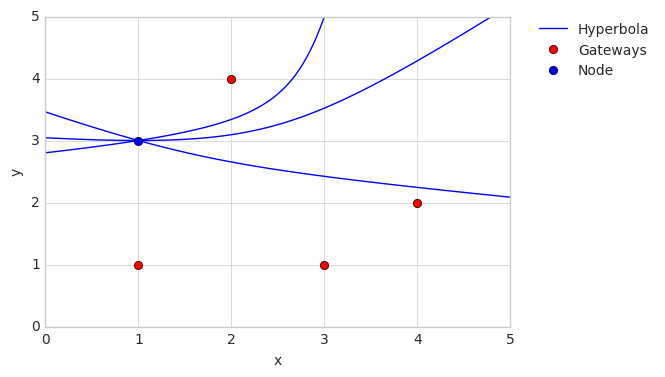
\includegraphics[width=12cm]{figures/TDOA.png}
      \caption{TDOA Hyperbola with 4 gateways}
      \label{fig:tdoa}
      \end{figure}

    \subsection{Hyperbolic Solver Algorithms}
      The non-linear nature of the set of hyperbolic TDOA equations \ref{eq:tdoa} means it is more difficult to solve for the node position than in trilateration techniques. A number of efficient methods exist that include both iterative and closed form algorithms \cite{ElGemayel2013}. Closed form algorithms are more computationally efficient and directly calculate exact solutions but cannot easily support over-determined situations \cite{Li2011}. Two such algorithms are Fang's \cite{Aatique1997} and Chan's \cite{Chan1994}. Iterative algorithms are popular and can take additional data in over-determined situations, with most based on the theory of least squares \cite{Koks2007}. They begin with an initial guess and improve the guess on each iteration. Gauss Newton is one such algorithm. Kalman filters are also popular methods for solving the set of equations.

    \subsection{Problems}
      Whilst TDOA is the best suited technique for locating using LoRaWAN, it is not without its hurdles \cite{LinkLabs}. One of the biggest is the assumption that there is minimal difference between the euclidean distance between the transmitting node and receiving gateways and the length of the propagation path, which is often unlikely in an urban environment and LoRaWAN is specifically designed to not require line of sight. The consequence is that the propagation time and distance will often be longer than the euclidean distance reducing the accuracy of the estimated location. Methods of reducing the NLOS error and identifying NLOS gateways have been explored \cite{Cong2001} and it is has been suggested that hybrid methods of TDOA with RSSI could be used to reduce the impact of both multipath effects and NLOS \cite{Lategahn2013}\cite{ElGemayel2013a}.

      The issues of timing accuracy have already been discussed and the importance of clock synchronization between gateways is clear. With no control over the existing gateway hardware, this will likely be a limiting factor in the accuracy obtained. Ideally a high resolution timestamp would be generated at the physical layer of the receiver \cite{Li2011}, with accurate clocks synchronized with a GPS reference time pulse. However, work has been carried out on reducing the need for synchronized clocks \cite{Li2014} and solving a set of unsynchronized TDOA measurements \cite{Burgess2014}.

      The last major issue which can limit the positional accuracy is the narrow bandwidth of the LoRa signals \cite{LinkLabs}. The ability to differentiate between two different signals depends on the signal bandwidth, with \(1/B\) giving the multipath resolution. Any signals that do not have a time difference greater than this cannot be differentiated, although there are methods of mitigating this. For example, with a typical LoRa bandwidth of 125kHz, the resolution would be \SI{8}{\micro\second}. In distance terms, multipath signals will not be resolved as being seperate unless the difference in path lengths is at least 2.4km. For this reason, many indoor positioning systems use Ultra Wideband (UWB) systems and attempts to perform wideband spreading with narrowband radios to replicate the accuracies achieved with UWB have been attempted \cite{Kempke2014}. However with such low resolution and potentially inaccurate timestamps from the gateways, this is unlikely to become relevant with the current infrastructure.

\chapter{Implementation}

  This chapter will describe the implemented test setup, ranging from the hardware through to the software and data gathering. The setup consists of a simple custom node, the existing Things Connected LoRaWAN infrastructure across London and custom server-side software. The node transmits its real location as calculated by the on-board GPS which is received by LoRaWAN gateways and uploaded to the server. These real coordinates of the transmission location can then be later compared to the estimated location by the multilateration algorithm.


  \section{Node Hardware}

    \begin{figure}
    \centering
    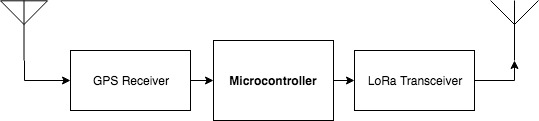
\includegraphics[width=12cm]{figures/node.jpeg}
    \caption{Node Diagram}
    \label{fig:node}
    \end{figure}

    A simple node was designed, built and programmed in C++, consisting of an ESP8266 microcontroller, u-blox MAX8C GPS receiver and a Microchip RN2483 LoRa transceiver, as shown in figure \ref{fig:node}. The RN2483 was chosen as it implements the full LoRaWAN stack on-board, reducing the complexity of the microcontroller code. The GPS receiver used a basic chip antenna whilst the LoRA transceiver used an 868MHz coiled helical antenna. The specific hardware is not particularly important however, but rather the functionality is.

    The GPS receiver was configured to pedestrian mode since the primary method of testing would be a person walking with the node, as opposed to a flight or high velocity mode which add filtering to improve accuracy in these scenarios. The LoRaWAN configuration parameters (device address, network session key and application session key) were hard-coded into the microcontroller firmware.

    The microcontroller follows a basic loop. In each iteration, set at roughly every 10 seconds, the microcontroller requests data from the GPS (latitude, longitude, altitude, number of satellites and time) and loads it into a struct datatype. A counter in the microcontroller's flash memory, such that it is persistent across power cycling, is incremented and also added to the struct. The entire 20 byte struct is then transmitted as a binary blob payload by the LoRa transceiver. Other functionality allowing transmission on a button press and short bursts of continuous data transmission was also implemented but not ultimately used.

    The main file of the node firmware can be seen in appendix \ref{ap:nodefirmware}. GPS interface code has been removed to a separate file and not included for brevity.


  \section{Server-side Software}

    \begin{figure}
    \centering
    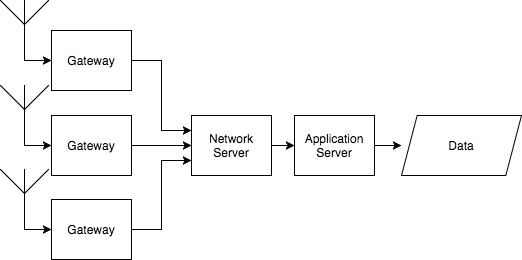
\includegraphics[width=12cm]{figures/server.jpeg}
    \caption{LoRaWAN to Server Diagram}
    \label{fig:server}
    \end{figure}

    When a gateway receives a packet from a node, it uploads it to the network server. The data can then be passed by the network server over an HTTP connection to the relevant application server, if the application server has implemented the necessary JSON-RPC methods \cite{EverynetAPI}. A python script to be run on a public server with open port 8080 is found in appendix \ref{ap:servereverynet} and implements the `uplink' and `post\_uplink' methods. The `uplink' method provides data as soon as one gateway has received a packet whilst the `post\_uplink' method should provide data on all receiving gateways a few seconds later. Unfortunately after testing, it was found that this latter method is not functional and that therefore obtaining details on all gateways is not possible this way. Hopefully it will be in the future.

    Therefore, a workaround was found by using the unofficial API running the Things Connected dashboard. The last 20 received packets from each gateway are available from a `messages' endpoint. By continuously polling this endpoint at a rate faster than that at which the node is transmitting, all data from all gateways can be collected. Figure \ref{fig:server} shows a simplified system diagram for the LoRaWAN and server-side systems. A python script to perform an HTTP POST request to login and continually fetch data from the unofficial API through HTTP GET requests is found in appendix \ref{ap:serverfetch}. The fetched data is published to a Redis Pub/Sub channel which is subscribed to by another script, found in appendix \ref{ap:serverprocess}, where the data is processed. The payload of each packet is decoded and the binary blob unpacked into the constituent pieces of data. If the packet payload already exists in the Redis database, the details of the new gateway receiving the packet is appended to the gateway list. If it doesn't already exist, the entire packet data is freshly inserted into the database.

    It is at this point in the system that any final positioning algorithm would ultimately be included. Instead, another python script, in appendix \ref{ap:serverexport}, allows all the received data to be exported from the database to a JSON file for analysis and testing.



\chapter{Data Analysis \& Results}

  In this chapter, the gathered data and the various transformations, algorithms and analytics carried out will be presented alongside the final positioning errors obtained. All investigations were programmed in Python and carried out in an iPython Jupyter notebook, with plots generated using matplotlib.

  \section{Gathered Data}

    The GPS node was taken for a walk through central London, through both areas with a high number and low number of gateways. Table \ref{tab:gatewaynums} shows the number of gateways that each packet was received by, with 648 packets received in total by 8 different unique gateways. It can be seen that only about 25\% of packets were received by 3 or more gateways, with three gateways being the minimum requirement to estimate a 2-dimensional position.

    Figure \ref{fig:datamap} provides a geographical visualization of the data. The location of each gateway that received a packet is shown in blue, the true location of packets received by less than 3 gateways are shown in red and the true location of packets received by 3 or more gateways are shown in green. With a cursory glance, it can be seen that generally more packets are received by higher numbers of gateways in areas of high gateway density.

    Taking a closer look at the received data, each gateway provides the latitude, longitude and altitude of its position and a timestamp with microsecond precision. Since the position coordinates for each gateway vary between packets, it would seem that for every packet received, a new location is retrieved from the GPS. It is unknown whether the timestamp is also retrieved live from the GPS, or from an internal clock. Either way, microsecond precision is not ideal bearing in mind that \SI{1}{\micro\second} is equivalent to 300 metres in distance. This also means it is unlikely the timestamping occurs at the instant a packet is first received.

    \begin{table}[ht]
      \begin{center}
        \caption{Number of packets received by n gateways}
        \label{tab:gatewaynums}
        \begin{tabular}{|c|c|c|c|c|c|c|}
          \hline
          Number of Gateways & 1 & 2 & 3 & 4 & 5 & Total \\
          \hline
          Number of Packets & 310 & 168 & 111 & 46 & 13 & 648 \\
          \hline
        \end{tabular}
      \end{center}
    \end{table}

    \begin{figure}[ht]
    \centering
    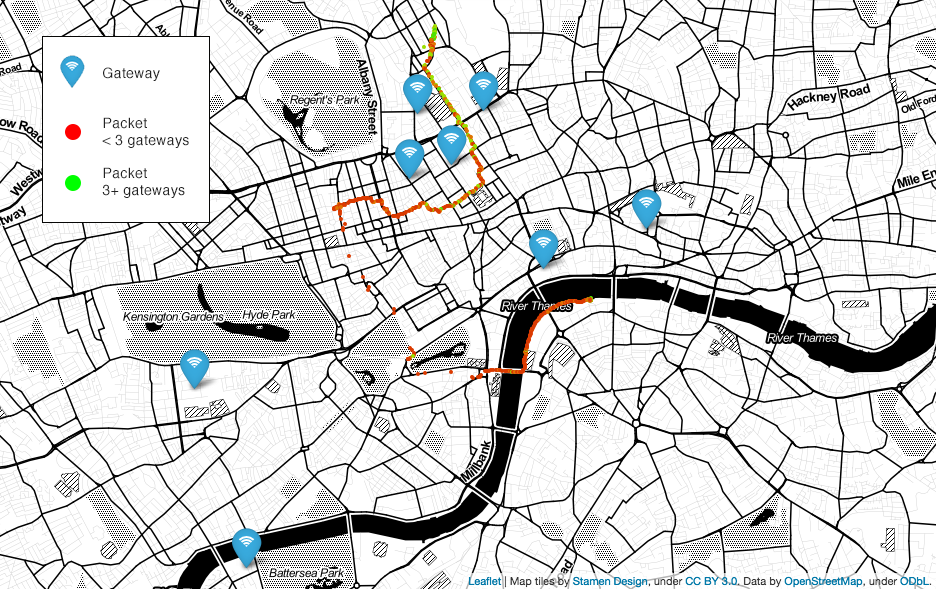
\includegraphics[width=15cm]{figures/map_data.png}
    \caption{Geographical visualization of gathered data}
    \label{fig:datamap}
    \end{figure}


  \section{Cartesian Coordinates}
    When working with the TDOA algorithms, it is important that a linear cartesian coordinate system is used, as opposed to the WGS84 latitude and longitude used by the GPS.

    If 3-dimensional positioning was required, latitude, longitude and altitude (LLA) could be converted to the Earth Centred, Earth Fixed (ECEF) frame and vice versa. In this reference frame, the origin is at the centre of the Earth with the x-axis intersecting the Greenwich meridian and the equator, the z-axis being along the spin axis of the Earth and the y-axis being perpendicular to both of these. However, for 3-dimensional position estimates, a minimum of 4 gateways would be required and the effect of altitude is likely to be negligible compared to other sources of errors.

    For 2-dimensional positioning, a local grid reference frame can be used. Latitude and longitude can be converted to OSGB36, the British Ordnance Survey National Grid reference system, and vice versa, through a number of calculations and adjustments detailed in OSTN02 \cite{OSTN02}. The resulting cartesian coordinates are in metres and also allow for easy plotting of the hyperbolic equations and position estimates. When positioning errors and distances are given, it is simply the euclidean distance between two sets of (x,y) coordinates in metres.

  \section{Received Signal Strength}

    The Received Signal Strength Indicator (RSSI) has already been discounted as a viable method of positioning due to the broad number of factors involved of which distance is only one. Figure \ref{fig:rssidistance} plots the RSSI of each packet received by each gateway against the distance from the transmission to the gateway. Whilst it can be seen that there is a relationship, the large variance of RSSI for any distance, particularly at the lower end, makes it unusable for positioning on its own.

    \begin{figure}[ht]
    \centering
    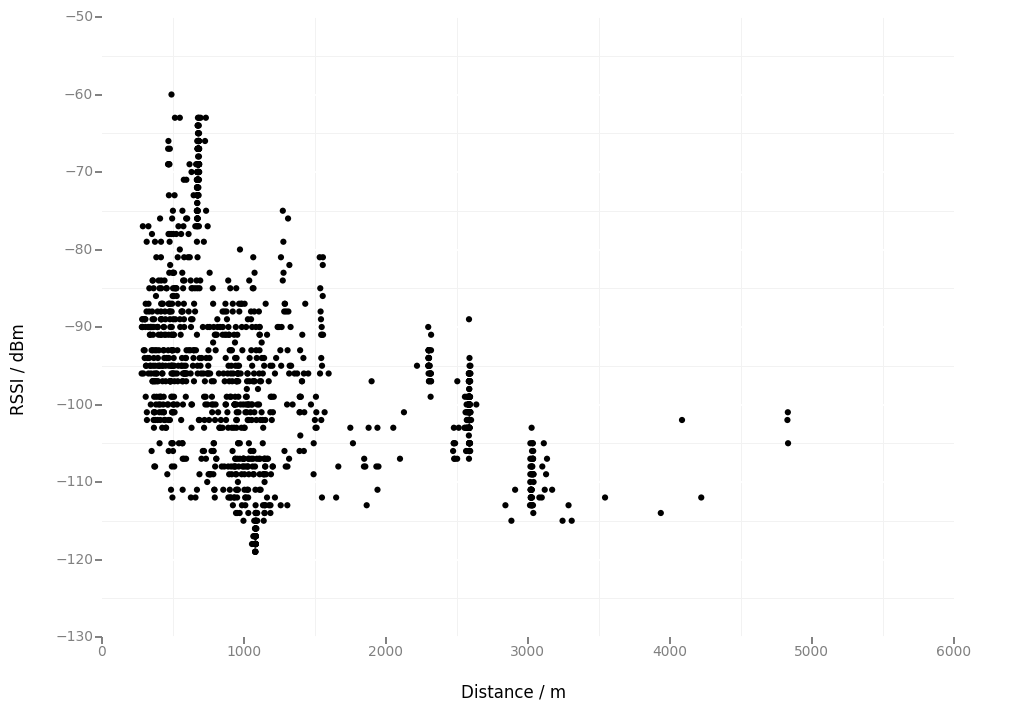
\includegraphics[width=15cm]{figures/rssidistance.png}
    \caption{Relationship between RSSI and distance from gateway}
    \label{fig:rssidistance}
    \end{figure}

  %\section{Data Cleanup}

  %  It was found after initial investigations and whilst programming Chan's algorithm that there were numerous issues with the data. The first issue is that some packets appeared to be received by one gateway more than once with varied receive times. Whether this is due to an issue with the particular gateway, or its location causing excessive multipath effects is unknown.

  \section{Chan's Algorithm}

    Initial investigations were carried out using an implementation of Chan's algorithm \cite{Chan1994}.

    The results of applying Chan's algorithm to the raw data directly, choosing the latter 3 gateways to have received each packet, were disappointing and can be seen in table \ref{tab:chanresults}. Out of 170 possible packets that were received by 3 or more gateways, the algorithm only returned position estimates for 18, or about 11\%. The mean positional error of these when compared to the true locations was 1112 metres.

    When the hyperbolic equations were plotted, it was found that the majority of packets did not have hyperbola that ever intersected or did not have hyperbola that were even valid due to the limited precision of the gateway timestamps. One such instance can seen in figure \ref{fig:hyperbolanointersect}. A limitation of Chan's algorithm is that it calculates exact solutions to the hyperbolic equations, so in all these instances where no exact solutions exist it was unable to provide a result.

    \begin{figure}[ht]
    \centering
    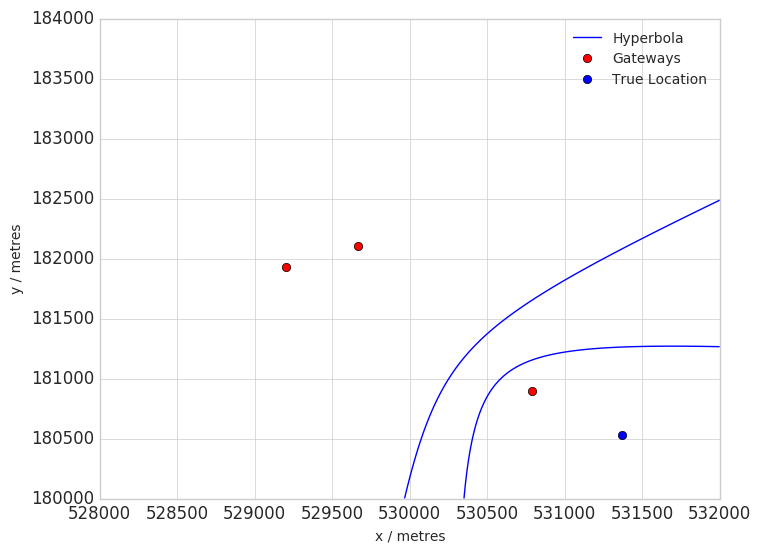
\includegraphics[width=10cm]{figures/hyperbolanointersect.png}
    \caption{Geographical plot of packet with non-intersecting hyperbola}
    \label{fig:hyperbolanointersect}
    \end{figure}

    \begin{table}[ht]
      \begin{center}
        \caption{Results of Chan's algorithm}
        \label{tab:chanresults}
        \begin{tabular}{|c|c|c|c|c|c|c|}
          \hline
           & Resolvable Packets & Mean Error & Median Error & Standard Deviation \\
          \hline
          Raw Data & 10.6\% & 1112m & 882m & 671m \\
          \hline
          Offsets & 17.0\% & 38,810m & 903m & 110,200m \\
          \hline
          Offsets (outliers removed) & 14.1\% & 866m & 642m & 767m \\
          \hline
        \end{tabular}
      \end{center}
    \end{table}

  \section{Offsets}

    In an attempt to improve the initial results achieved with Chan's algorithm, both in terms of the number of packets with a solution and in terms of the positional error, it was theorized that each gateway may have a timing offset associated with it which could be corrected for. This is similar to the Differential TDOA approach \cite{Li2014} which uses a reference node to compensate for imperfect synchronization between gateways. Offsets cannot be calculated for each gateway individually since we are using TDOA and do not have an exact transmit time, but offsets for pairs of gateways can be found.

    The offset of a pair of gateways, i and j, is shown in equation \ref{eq:offset}. The result of the difference of the euclidean distances from the true position of the packet, \(d_i - d_j\), divided by the speed of light, C, is what the time difference of arrival should be. Therefore the difference of this value and the TDOA, \(t_i - t_j\), provides a time offset for that pair of gateways.

    \begin{equation}
    \label{eq:offset}
    offset_{ij} = (\frac{d_i - d_j}{C}) - (t_i - t_j)
    \end{equation}

    The offset is calculated for every possible pair of gateways for every packet. The probability density function (PDF) for these offsets is shown in figure \ref{fig:offsetpdf} and it can be seen that they are quite varied, with the majority of values within \SI{10}{\micro\second} and the mean at \SI{3.58}{\micro\second}. In terms of distance, that is a mean offset of over 1km.

    \begin{figure}[ht]
    \centering
    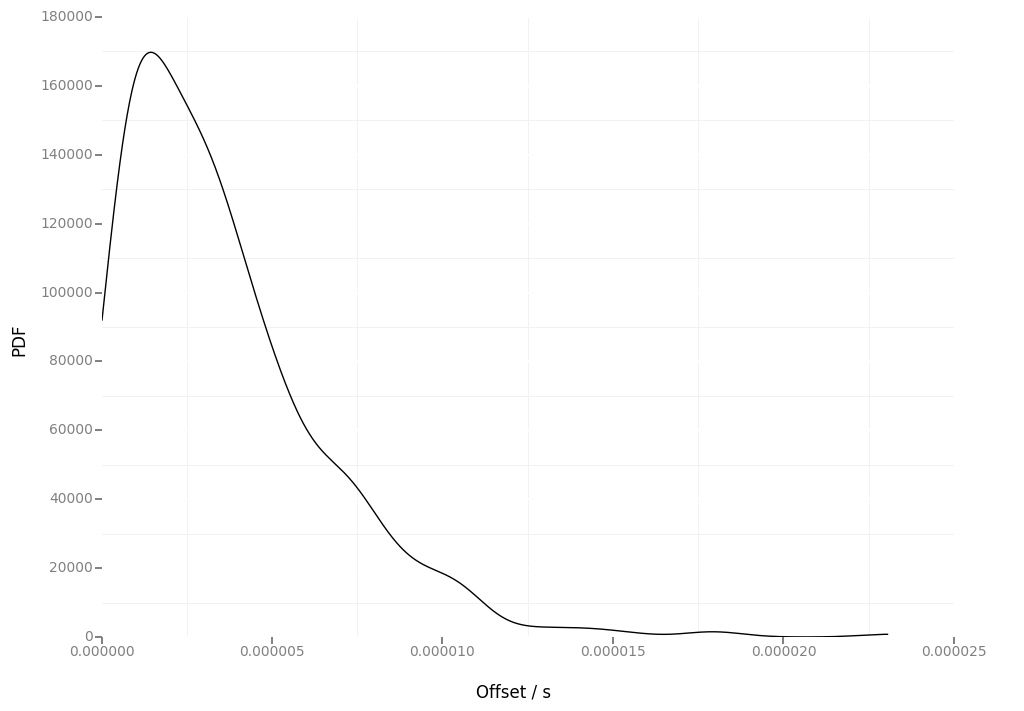
\includegraphics[width=12cm]{figures/offsetpdf.png}
    \caption{Probability Density Function for all calculated offsets}
    \label{fig:offsetpdf}
    \end{figure}

    \begin{figure}[ht]
    \centering
    \begin{subfigure}[b]{7cm}
        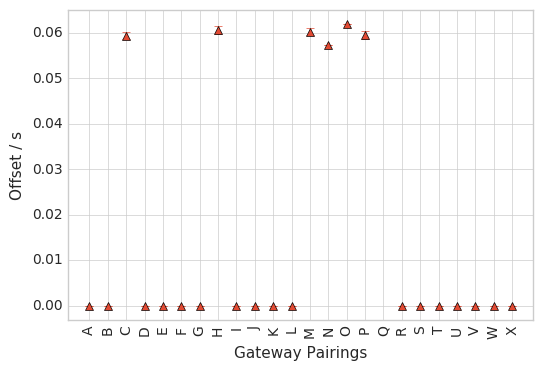
\includegraphics[height=5cm]{figures/offsetsall.png}
        \caption{All gateway pairs}
        \label{fig:offsetboxesa}
    \end{subfigure}
    ~
    \begin{subfigure}[b]{7cm}
        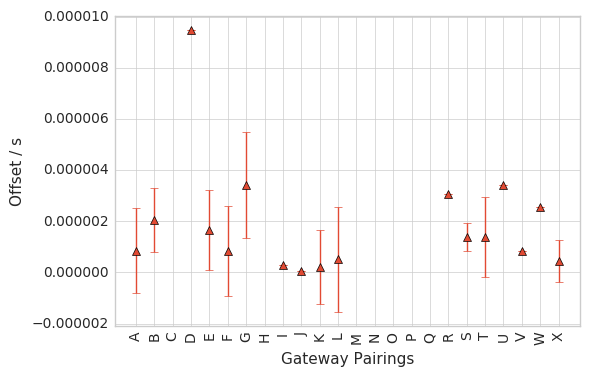
\includegraphics[height=5cm]{figures/offsetssmall.png}
        \caption{Gateway pairs with \si{\micro\second} offsets}
        \label{fig:offsetboxesb}
    \end{subfigure}
    \caption{Mean and Standard Deviations of Calculated Offsets} \label{fig:offsetboxes}
    \end{figure}

    Of greater significance are the spread of values for each individual pairing, shown in figures \ref{fig:offsetboxesa} and \ref{fig:offsetboxesb}. \ref{fig:offsetboxesa} shows that some pairings have mean offsets of as high as 0.06s, which would cause significant errors in positioning and likely cause no solution to be found at all. \ref{fig:offsetboxesb} narrows down to those pairings with offsets in the microsecond range and allows the standard deviation bars to be seen. These show that the offsets are not particularly constant for most pairings, perhaps suggesting that other factors are involved such as multipath and non-line-of-sight effects or just that the gateways do not assign a timestamp in a particularly controlled way.

    Applying these mean offsets to the TDOAs before using Chan's algorithm results in slight improvements with a solution for 17\% of packets, shown in row 2 of table \ref{tab:chanresults}. Due to clear outliers however, resulting in solutions tens of kilometres from the gateways, the mean positional error is almost 40km but with a median of only 903m. Removing these outliers gives solutions for about 14\% of packets with a mean positional error of 866m, shown in row 3 of table \ref{tab:chanresults}, down from an error of 1112m without applying offsets.


  \section{Iterative Algorithm}

    Even with the addition of offsets, Chan's algorithm severely limits the number of resolvable packets. Ideally an approximate solution is needed in the cases when the hyperbolic equations do not intersect and this is provided by utilizing an iterative algorithm rather than a closed. With the implementation of a least squares based iterative algorithm, an exact solution does not need to exist. In addition, all the data in over-determined situations can more easily be used, potentially improving the estimation accuracy - i.e. when there are more than 3 gateways that have received a packet and thus more TDOA equations than there are unknown coordinates. Being an iterative algorithm, an initial estimate is required and the further the estimate from the true solution, the more iterations it will take to converge on a solution. To keep processing times down, a limit on the number of iterations will normally be set and so ideally the initial estimate will be set to be as close to the solution as possible. With trial and error of several potential initial estimates, including using the origin (0,0) and the result of the previous estimate, it was found that using the position of the first receiving gateway minimized the number of packets which did not converge. The only other possible disadvantage of an iterative technique compared to a closed form algorithm such as Chan is the processing time - however, the processing is being performed on the server-side rather than an embedded device and so this an inconsequential issue.

    When the iterative algorithm was run on the raw data, the results were immediately an improvement with a solution returned for about 44\% of packets that were received by three or more gateways, compared to 14\% with reasonable error for Chan's algorithm. As shown in row 1 of table \ref{tab:iterresults}, the mean positional error achieved was 972m, a similar figure to Chan's.

    Since all receiving gateways are taken into account using the iterative algorithm, improvements were found by rejecting outliers in the receiving gateway timestamps. Erroneous times that would clearly put the node beyond the reach of the network were rejected, resulting in solutions for over 58\% of packets with a mean positional error of just over 1km, shown in row 2 of table \ref{tab:iterresults}. By also applying the offsets for gateway pairs before using the iterative algorithm, solutions were found for about 55\% of packets with a mean positional error of 930m and a lower standard deviation of 557m, shown in row 3 of table \ref{tab:iterresults}.

    \begin{table}[ht]
      \begin{center}
        \caption{Results of Iterative algorithm}
        \label{tab:iterresults}
        \begin{tabular}{|c|c|c|c|c|c|c|}
          \hline
           & Resolvable Packets & Mean Error & Median Error & Standard Deviation \\
          \hline
          Raw Data & 44.1\% & 972m & 850m & 614m \\
          \hline
          Raw Data (reject outliers) & 58.2\% & 1080m & 929m & 716m \\
          \hline
          Offsets & 55.3\% & 930m & 863m & 557m \\
          \hline
        \end{tabular}
      \end{center}
    \end{table}

    To better visualize the positional error, figure \ref{fig:iterrorcdf} plots the cumulative density function for the iterative algorithm. Whilst the mean error for all three sets of results are around 1km, the variability of the positional error is large with errors as great as 3km occurring. It is seen again that including offsets provides slightly better results, with a 1440m accuracy at 80\% confidence level. The raw data with outliers rejected is interestingly the worst, with 1720m accuracy at 80\% confidence and ordinary raw data at 1510m accuracy - though it must be remembered that the ordinary raw data achieved a lower number of resolvable packets. Ultimately though, all three curves are very similar and so precise and reliable positioning would therefore appear to be beyond the scope of the current network, but a rough position over a broad city scenario can certainly be achieved.

    \begin{figure}[ht]
    \centering
    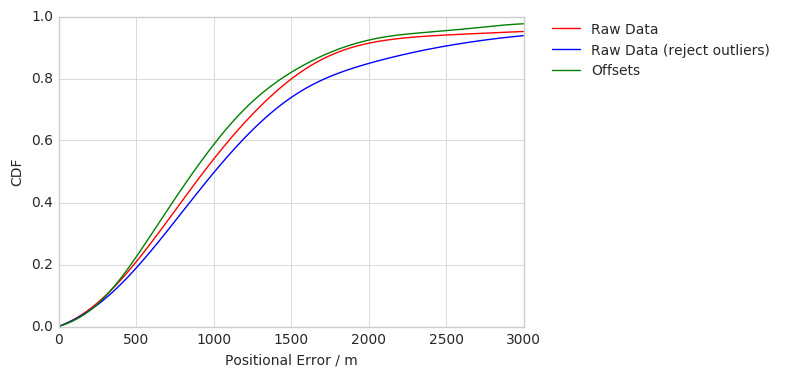
\includegraphics[width=14cm]{figures/iterativecdf.png}
    \caption{Cumulative Distribution Function for Positional Error using Iterative Algorithm}
    \label{fig:iterrorcdf}
    \end{figure}


  \section{Oversampling}

    Lastly, oversampling was employed in an attempt to improve the positional accuracy and reduce noise. With the test node stationary at one location known to be picked up by multiple gateways, a large number of transmissions were made. Two methods were considered to test the viability of oversampling, the first being to calculate every possible TDOA and find the mean for each gateway pair to achieve a higher resolution time difference. The second was to find an estimated location for every packet and take the mean of the coordinates as the final estimate. This latter method was chosen as simpler and likely to produce similar results.

    \begin{table}[ht]
      \begin{center}
        \caption{Results of Oversampling with Iterative algorithm}
        \label{tab:osresults}
        \begin{tabular}{|c|c|c|>{\bfseries}c|}
          \hline
           & Resolvable Packets & Mean Error &  Final Estimate Error \\
          \hline
          Data & 29\% & 1196m & 467m \\
          \hline
          Data (reject outliers) & 64\% & 1198m & 392m \\
          \hline
        \end{tabular}
      \end{center}
    \end{table}

    Running the iterative algorithm on each individual packet received from the location resulted in a mean positional error of almost 1.2km with only 29\% of packets achieving a solution. However, the mean location calculated from the set of estimated coordinates achieved a far lower positional error of just 467m, shown in row 1 of table \ref{tab:osresults}.

    Running the algorithm again whilst rejecting outliers resulted in a mean positional error of almost 1.2km but with 64\% of packets achieving a solution. With more packets therefore being using to estimate the final location, a positional error of 392m is found, shown in row 2 of table \ref{tab:osresults}. These results are visualized in figure \ref{fig:oversampleplot}, where the individual location estimates can be seen with the final estimated location in green and true location in blue.

    Whilst these results are promising and more accurate than estimating locations based on an individual transmission, this method is likely only suitable for use on stationary nodes. Whilst transmitting multiple packets in bursts is possible, it is undesirable both due to power constraints and sharing use of the network amongst potentially large numbers of other nodes. In reality, any oversampling of location will happen over longer periods of time, reducing usefulness for moving nodes which are the primary use case for positioning.

    \begin{figure}[ht]
    \centering
    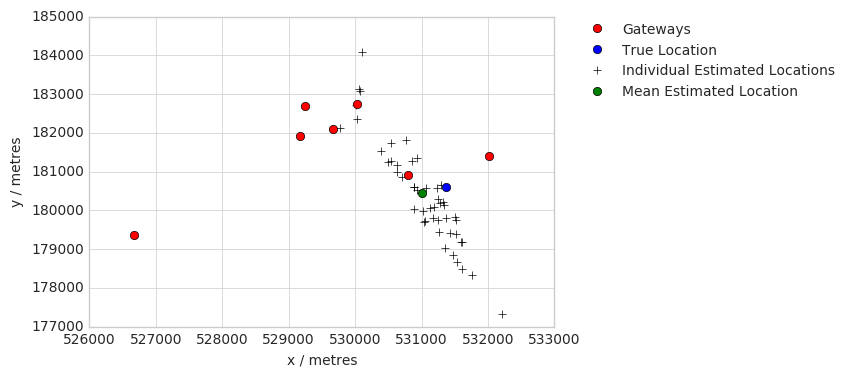
\includegraphics[width=16cm]{figures/oversampleplot.png}
    \caption{Geographical plot of oversampling with iterative algorithm}
    \label{fig:oversampleplot}
    \end{figure}



\chapter{Conclusion}

  With the huge growth rate of the Internet of Things and broad range of applications, it is clear that positioning will be a key requirement for many devices. As LoRaWAN too increases in popularity due to its long range, ease of use and low costs and low power consumption for connected devices, locating these devices without giving up any one of these becomes highly desirable.

  It was decided that using the Time Difference of Arrival between pairs of gateways was the most viable approach and using an iterative algorithm was found to provide better results than a closed form solution for the collected data, but ultimately only coarse positioning estimates were able to be obtained. The smallest mean positional error was 930m, with the smallest accuracy being 1440m at an 80\% confidence level. With only 25\% of packets being received by 3 or more gateways and only just over half of these resulting in position estimates, it is clear that LoRaWAN as it currently stands could be suitable for general positioning over large areas but not for applications that require reliability or accuracy.

  It was found that calculating offsets for pairs of gateways did improve the positional accuracy, however they had large variances likely due to both NLOS transmissions and the way in which timestamping is implemented in the gateways. Ideally offsets could be calculated on solely LOS transmissions allowing for the quantification of the effects of NLOS on accuracy. Cross validation should also be performed on a larger dataset since it is possible that the small improvements found were due to overfitting of the offsets to the data, particularly in the case of gateway pairs with only a few transmissions.

  Oversampling of transmissions from a stationary node did appear to cause significant improvements in accuracy, down to a positional error of just 400m. However most applications for location estimates in the IoT will not be stationary. Bursts of transmissions in a short space of time may help for slow moving devices, but this is undesirable for low power devices and particularly in a network with many transmitting devices.

  It is important to note, however, that the Things Connected network tested is relatively new and that with a broader spread of gateway locations, the numbers of receiving gateways are likely to be improved. It should also be noted that investigating the number of receiving gateways and distance from gateways was not a primary aim and ideally more data representing a greater geographical spread around the network's gateways would be collected and thus the reliability of these statistics improved.

  With more gateways that are more evenly distributed, there would also be a higher proportion of transmissions that are closer to being LOS, reducing the error due to NLOS paths. A higher proportion of packets would also be picked up by 3 or more gateways, providing a better conversion rate of transmissions to location estimates. Femto LoRaWAN gateways have been suggested to provide increased coverage in urban environments, particularly aiding positioning \cite{Lestable}. Combined RSSI and TDOA techniques could also be investigated, with the potential for utilizing machine learning with increased data.

  Ideally though, the gateway hardware would be improved to provide accurate, precise timestamps at the physical layer. Synchronizing the gateway clock with a reference time pulse from GPS and assigning a time of arrival to a packet as the signal first arrives will greatly improve accuracy, rather than carrying out timestamping in the less time critical MAC layer which it is suspected is currently the case.


% Bibliography
\bibliographystyle{IEEEtran}
\bibliography{references}

% Appendix
\appendix
\chapter{Node Firmware} \label{ap:nodefirmware}
  \lstinputlisting[language=C++, basicstyle=\small]{nodecode.ino}

\chapter{Server-Side Software}
  \section{Python Everynet API Script} \label{ap:servereverynet}
    \lstinputlisting[language=Python, basicstyle=\small]{everynetapi.py}

  \newpage
  \section{Python Fetch Script} \label{ap:serverfetch}
    \lstinputlisting[language=Python, basicstyle=\small]{dashboard_fetch.py}

  \newpage
  \section{Python Processing Script} \label{ap:serverprocess}
    \lstinputlisting[language=Python, basicstyle=\small]{process_messages.py}

  \newpage
  \section{Python Export Script} \label{ap:serverexport}
    \lstinputlisting[language=Python, basicstyle=\small]{export_data.py}


\end{document}
